\documentclass[12pt,a4]{article}
\usepackage{physics, amsmath,amsfonts,amsthm,amssymb, mathtools,steinmetz, gensymb, siunitx}	% LOADS USEFUL MATH STUFF
\usepackage{xcolor,graphicx}
\usepackage[left=45pt, top=20pt, right=45pt, bottom=45pt ,a4paper]{geometry} 				% ADJUSTS PAGE
\usepackage{setspace}
\usepackage{caption}
\usepackage{tikz}
\usepackage{pgf,tikz,pgfplots,wrapfig}
\usepackage{mathrsfs}
\usepackage{fancyhdr}
\usepackage{float}
\usepackage{array}
\usepackage{booktabs,multirow}
\usepackage{bm}

\usetikzlibrary{decorations.text, calc}
\pgfplotsset{compat=1.7}

\usetikzlibrary{decorations.pathreplacing,decorations.markings}
\usepgfplotslibrary{fillbetween}

\newcommand{\vect}[1]{\boldsymbol{#1}}

\usepackage{hyperref}
%\usepackage[style= ACM-Reference-Format, maxbibnames=6, minnames=1,maxnames = 1]{biblatex}
%\addbibresource{references.bib}


\AtBeginDocument{\hypersetup{pdfborder={0 0 0}}}

\title{
\textsc{Topic 2}
}
\author{\textsc{J L Gouws}
}
\date{\today
\\[1cm]}



\usepackage{graphicx}
\usepackage{array}




\begin{document}
\thispagestyle{empty}

\maketitle

\begin{enumerate}
  \item
    \begin{enumerate}
      \item
        Figure~\ref{fig:1a} shows the forward Euler method's solution to the logistic problem in Eq.~\ref{eq:logit}.
        \begin{equation}
          \dot u = u (1 - u), \qquad \qquad u(0) = 0.05
          \label{eq:logit}
        \end{equation}
        \begin{figure}[H]
          \centering
          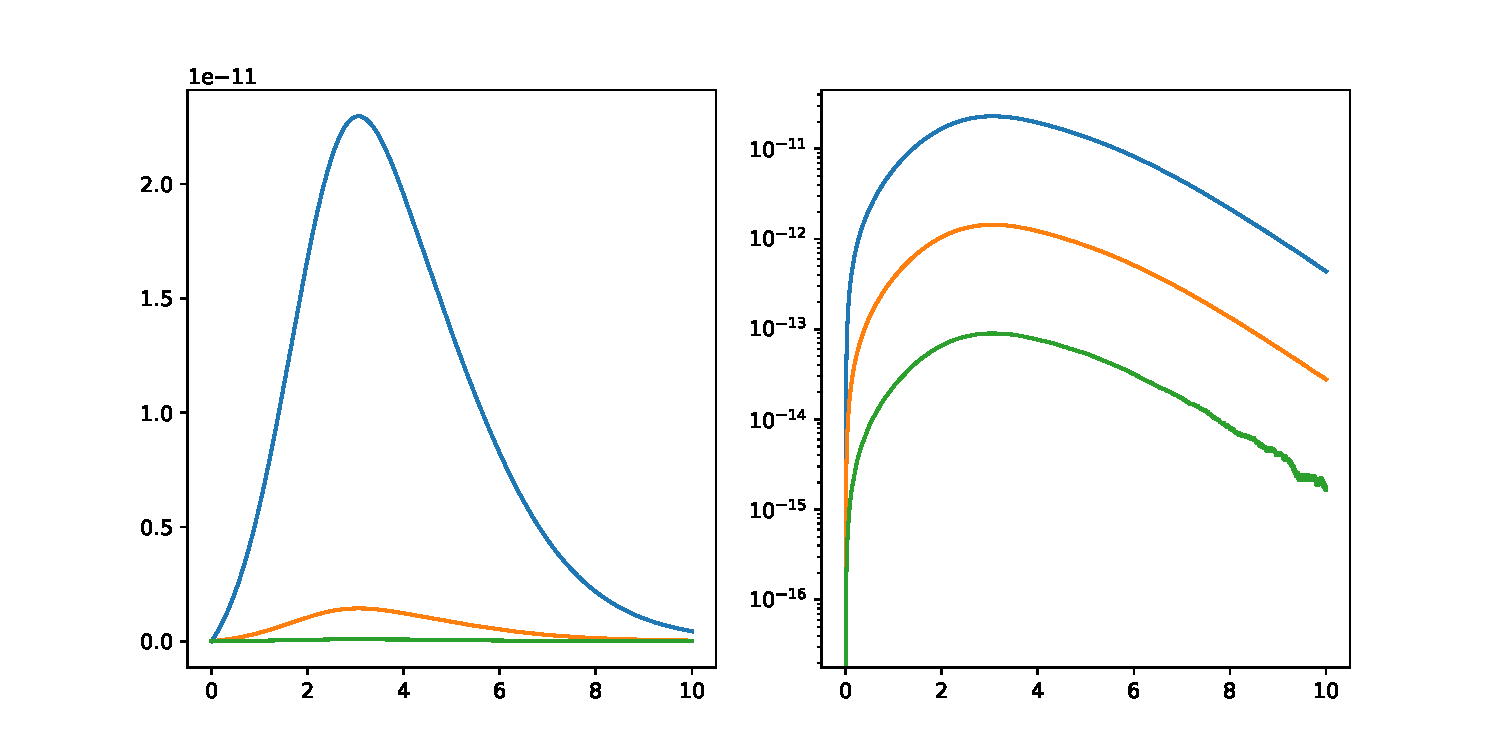
\includegraphics[scale = 0.8]{../figs/1a.pdf}
          \caption{Forward Euler solution of a logistic problem}
          \label{fig:1a}
        \end{figure}

      \item
        Figure~\ref{fig:1b} shows the midpoint method's solution to the logistic problem in Eq.~\ref{eq:logit}.

        \begin{figure}[H]
          \centering
          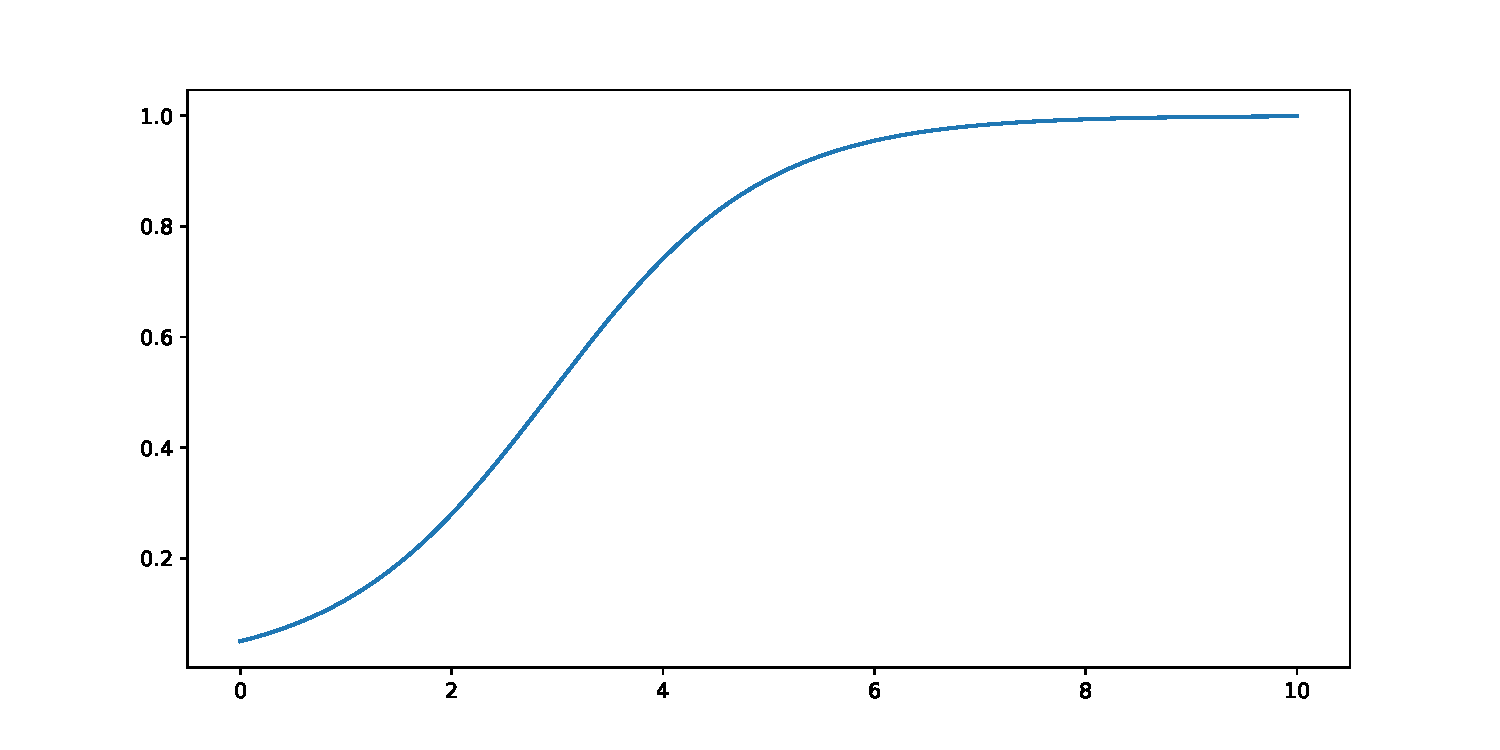
\includegraphics[scale = 0.8]{../figs/1b.pdf}
          \caption{Midpoint method solution of a logistic problem}
          \label{fig:1b}
        \end{figure}

      \item
        Figure~\ref{fig:1c} shows an RK2 method's solution to the logistic problem in Eq.~\ref{eq:logit}.
        \begin{figure}[H]
          \centering
          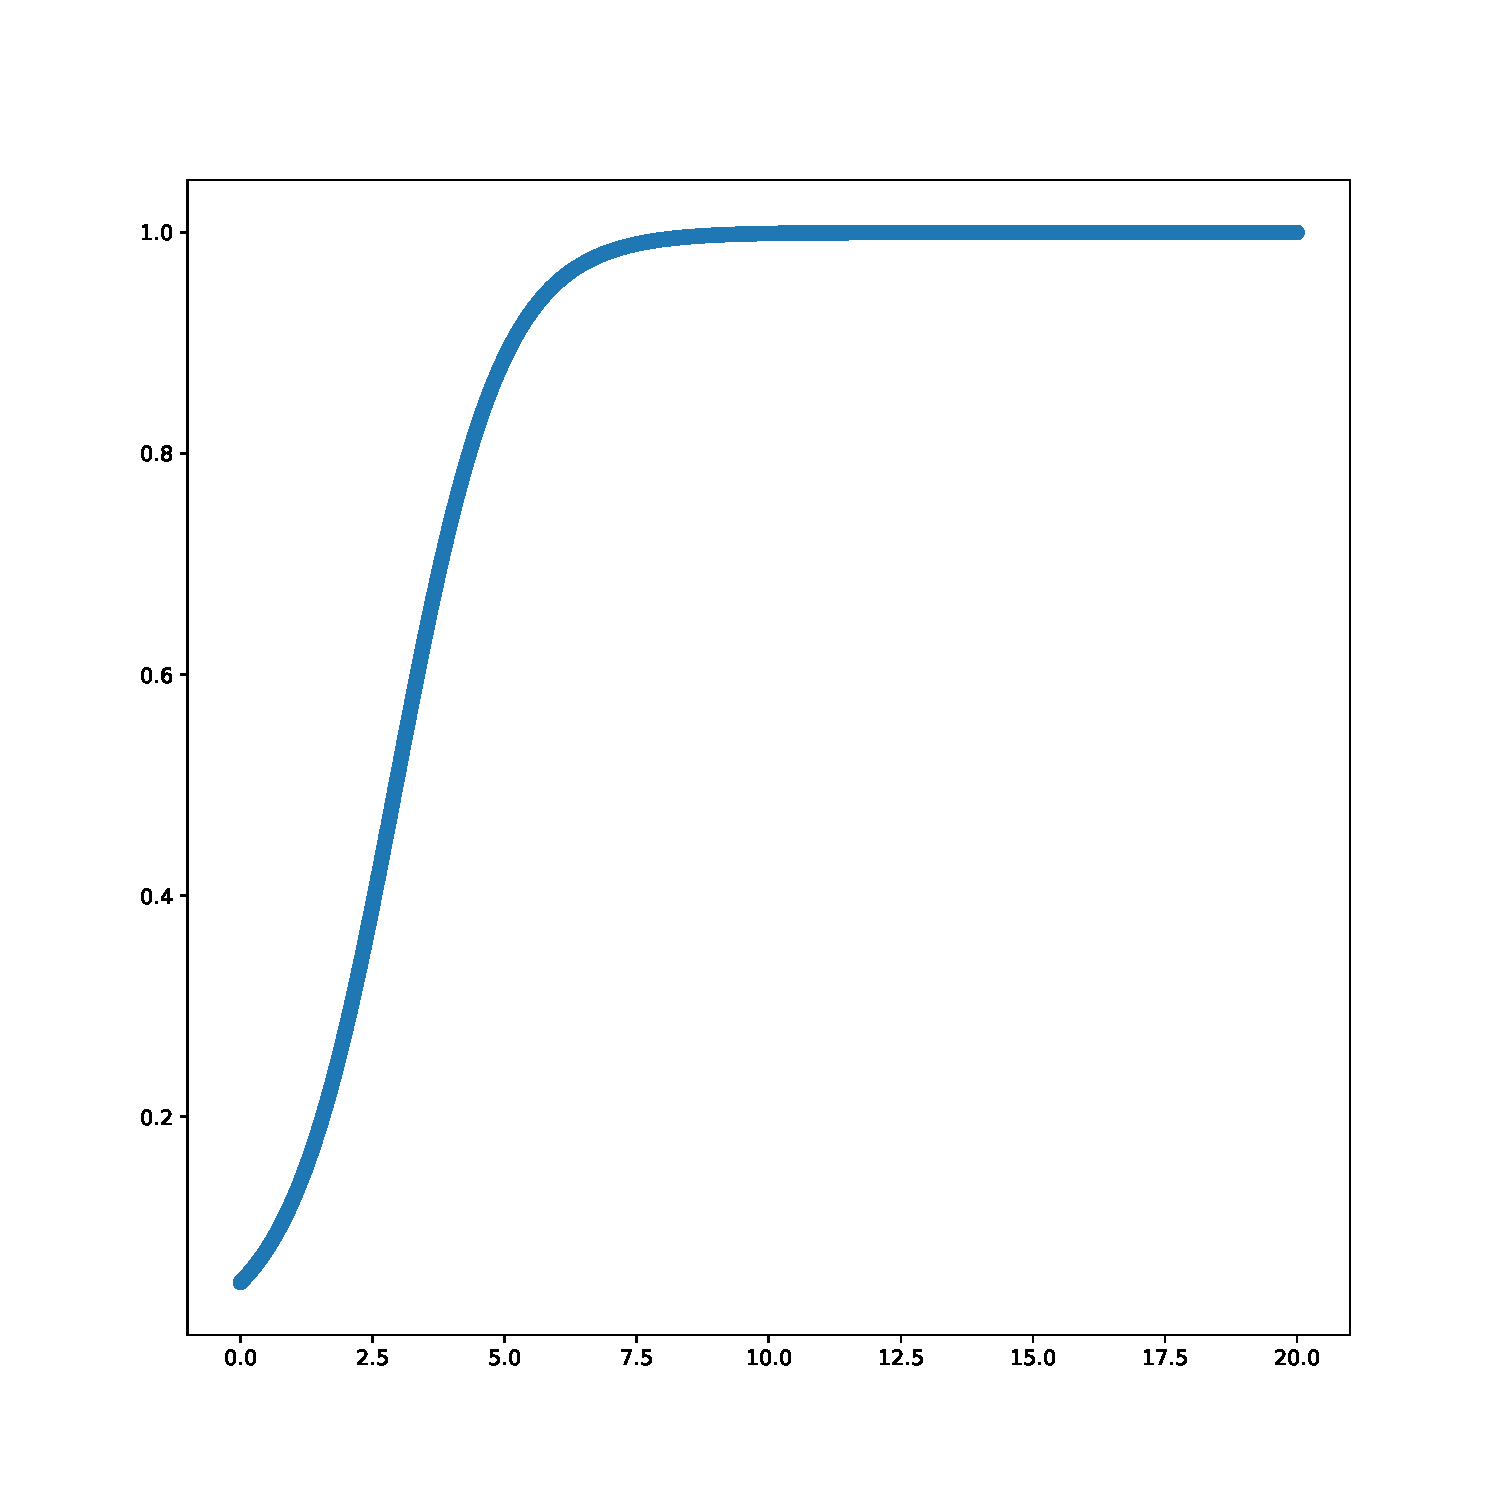
\includegraphics[scale = 0.8]{../figs/1c.pdf}
          \caption{RK2 Method solution of a logistic problem}
          \label{fig:1c}
        \end{figure}

    \end{enumerate}
  \item
    Figure~\ref{fig:2} shows solutions to the logistic equation in Eq.~\ref{eq:logit} for various initial conditions using an RK2 evolver.
    \begin{figure}[H]
      \centering
      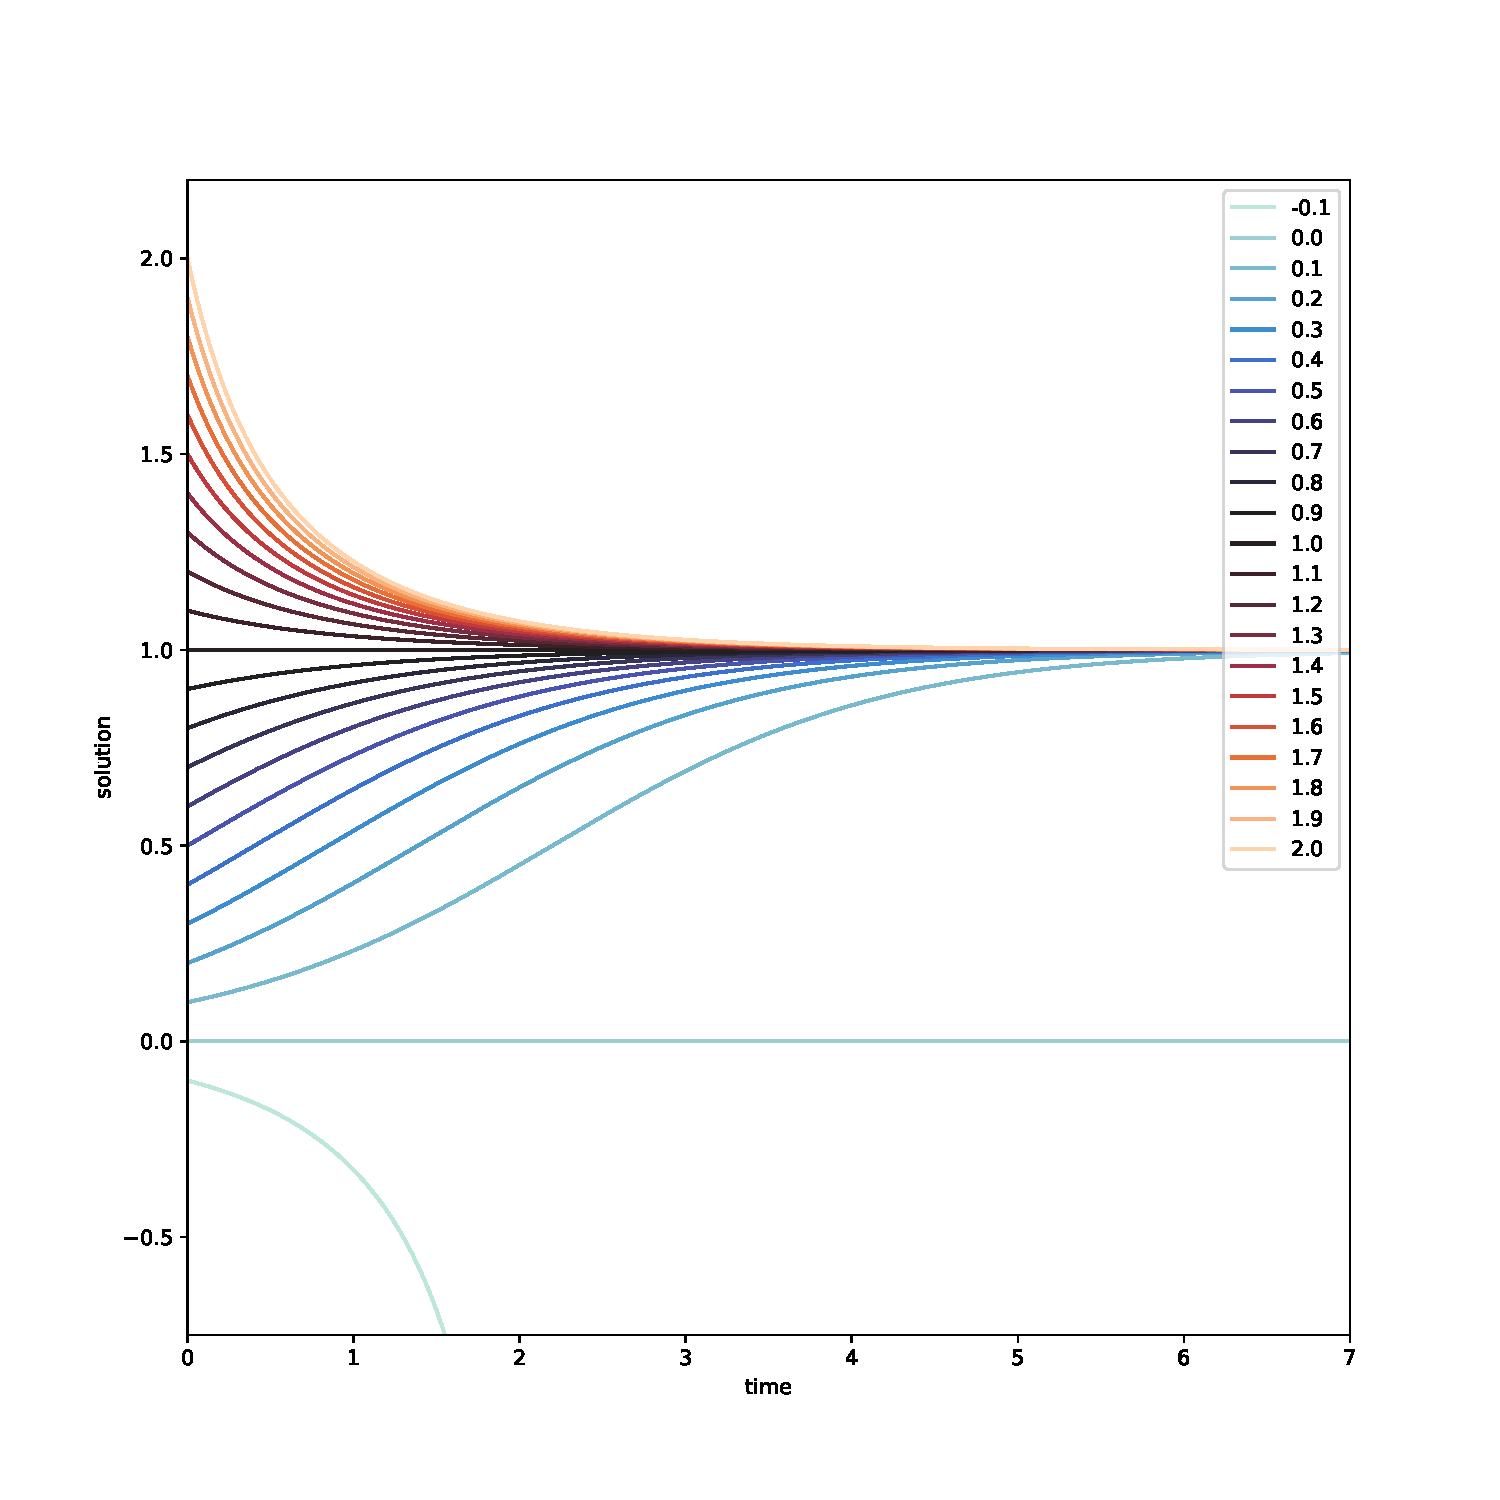
\includegraphics[scale = 0.6]{../figs/2.pdf}
      \caption{RK2 solutions to the logistic equation for various initial conditions}
      \label{fig:2}
    \end{figure}

     Figure~\ref{fig:2} suggests that the equilibrium points are at $u = 1$ and $u = 0$.
     The theory similarly states:
     \begin{equation*}
       u(1 - u) = 0 \Rightarrow u = 0 \text{ or } u = 1
     \end{equation*}
     The equilibrium point at $u = 0$ is unstable because:
     \begin{equation*}
       \left.\frac{d}{d u}u(1 - u) \right|_{u = 0} = 1 > 0
     \end{equation*}

     The equilibrium point at $u = 1$ is stable because:
     \begin{equation*}
       \left.\frac{d}{d u}u(1 - u) \right|_{u = 1} = -1 < 0
     \end{equation*}

  \item
    Figure~\ref{fig:3a} shows solution to the problem in Eq.~\ref{eq:3} using various methods and different time steps.
    \begin{equation}
      \dot u = u \frac{1}{2} e^{t / 2} \sin(5 t) + 5 e ^{t / 2} \cos(5 t), \qquad u(0) = 0
      \label{eq:3}
    \end{equation}
    \begin{figure}[H]
      \centering
      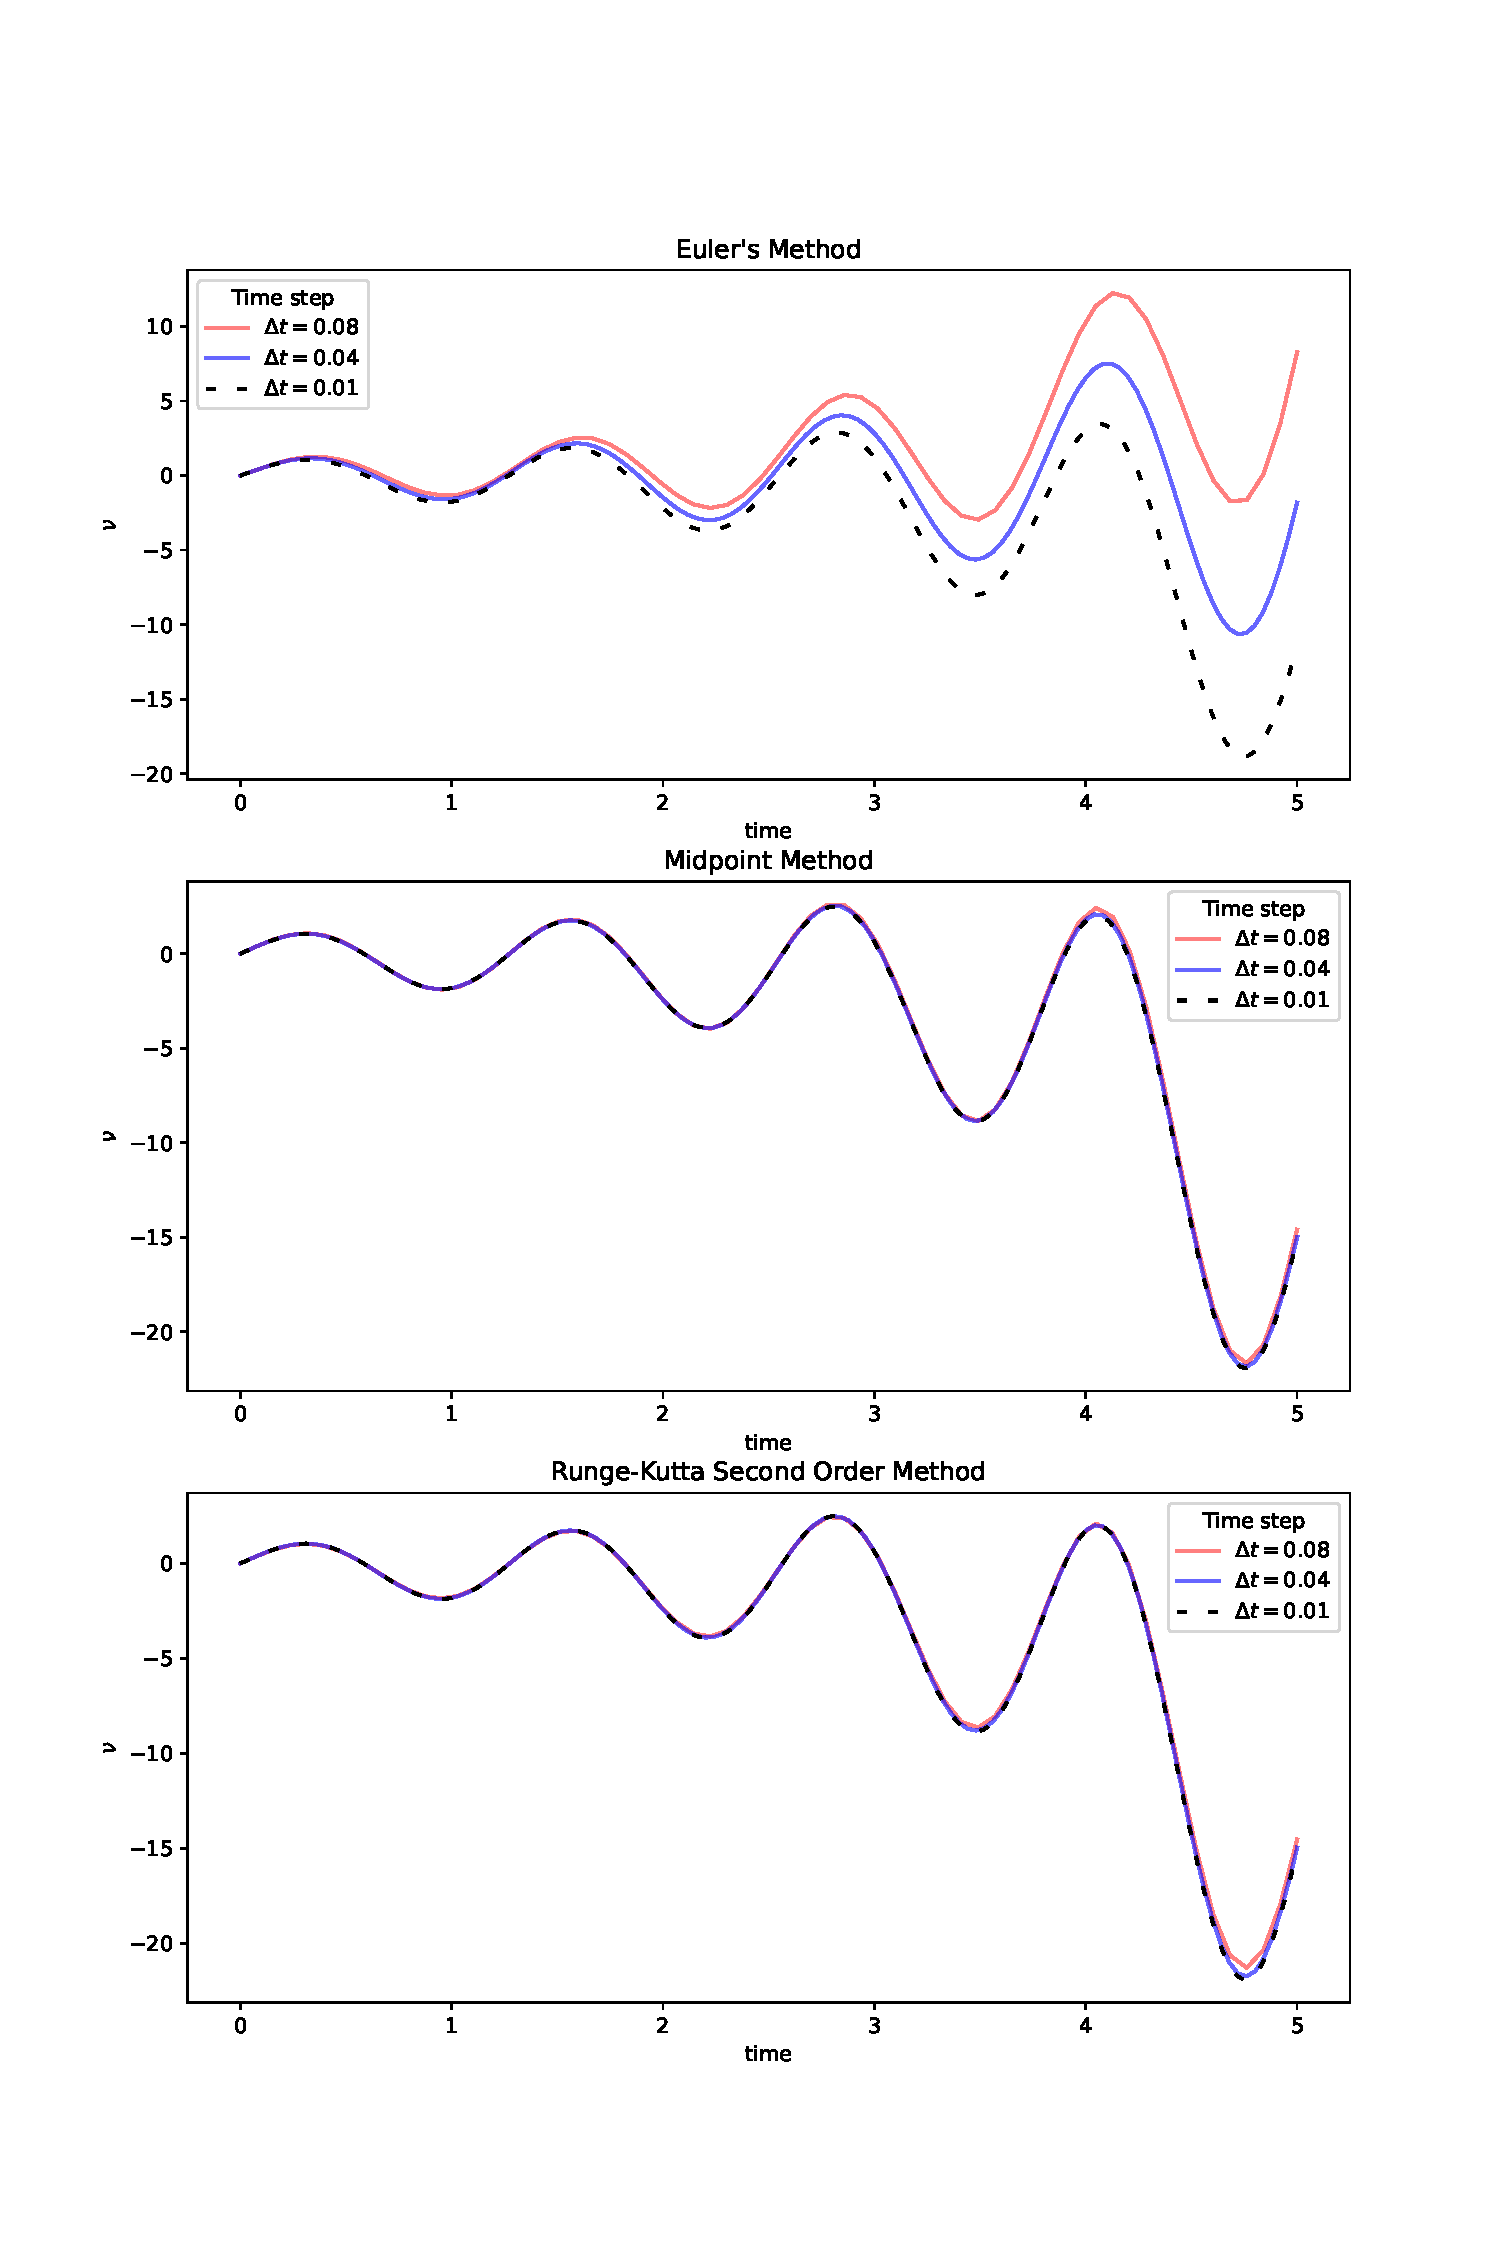
\includegraphics[scale = 0.7]{../figs/3a.pdf}
      \caption{Euler, midpoint and RK2 method solutions to a first order ODE using different time-steps}
      \label{fig:3a}
    \end{figure}
\end{enumerate}

\end{document}
